\documentclass{beamer}

\mode<presentation>
{
  \usetheme{CambridgeUS}
  \setbeamercovered{transparent}
}

\usepackage[T1]{fontenc}
\usepackage[utf8]{inputenc}
\usepackage[spanish]{babel}
\usepackage{color}
\usepackage{hyperref}
\usepackage{algorithm,algorithmic}
\usepackage{colortbl}
\usepackage{graphicx}
\usepackage{minted}

\usepackage[skins,minted]{tcolorbox}

\setminted[java]{
  linenos=true,
  fontfamily=tt,
  fontsize=\small,
  frame=leftline
}

\newtcblisting{java}[2][]{minted language=java,
  enhanced, listing engine=minted,
  listing only, #1, title=#2, left=2em
}

\setminted[bash]{
  linenos=true,
  fontfamily=tt,
  fontsize=\small,
  frame=leftline
}

\newtcblisting{bash}[2][]{minted language=bash,
  enhanced, listing engine=minted,
  listing only, #1, title=#2, left=2em
}




\usepackage{enumitem}
\setitemize{itemsep=1.2em,%
  label=\usebeamerfont*{itemize item}%
        \usebeamercolor[fg]{itemize item}%
        \usebeamertemplate{itemize item}
}

\title[\textbf{Programación 2}]{\textbf{Programación 2}}

\subtitle{Introducción a la Orientación a Objetos}
 
\author[IF-EG]
{
  Profesores:\\
  Ismael Figueroa -  \texttt{\small ifigueroap@gmail.com}\\
  \vspace{0.5mm}
  Eduardo Godoy - \texttt{\small eduardo.gl@gmail.com}
}

\institute[Universidad de Valparaíso]

\date{}

\begin{document}

\begin{frame}
  \titlepage
\end{frame}

\section{El Lenguaje de Programación Java}

\subsection{Antecedentes Generales}

\begin{frame}
  \frametitle{Inicio de Java}

    \begin{itemize}
    \item \textbf{Desarrollado por:} Sun Microsystems en 1991.
    \item \textbf{Propietario actual:} Oracle Corporation desde 2010.
    \item \textbf{Objetivo inicial y actual:}
      
      \begin{itemize}
      \item Desarrollar un lenguaje de programación para crear
        software peque\~nos, rápidos, eficientes y portátiles para
        diversos dispositivos de hardware (teléfonos celulares,
        radiolocalizadores y asistentes digitales personales).
        
      \item Ser el nexo universal que conecte a los usuarios con la
        información que esté situada en el computador local, en un
        servidor Web o en una base de datos.
      \end{itemize}
      
    \item \textbf{Principio:} \emph{Write Once, Run Everywhere}
      
    \end{itemize}    

\end{frame}

\begin{frame}
  \frametitle{Independencia de la Plataforma}
  
    \begin{itemize}
    \item \textbf{Tanto a nivel del código fuente como del binario.}



      \item \emph{\bf Independencia en código fuente}: los tipos
        primitivos de datos de Java tienen tama\~no consistentes en
        todas las plataformas de desarrollo. Las bibliotecas de Java
        facilitan la escritura del código, que puede desplazar se
        plataforma a plataforma.

      \item \emph{\bf Independencia en binario}: los archivos binarios
        (bytecodes) pueden ejecutarse en distintas plataformas sin
        necesidad de volver a compilar la fuente.
        
        % \begin{itemize}
        %	\item bytecodes: conjunto de instrucciones maás abstracto que el código máquina (código intermedio), pero no son especificas a un procesador.
        % \end{itemize}
      
    \end{itemize}
  
\end{frame}

\begin{frame}
  \frametitle{Ventajas}
    \begin{itemize}
    \item Fomenta la reutilización y extensión del código.
    \item Permite crear sistemas más complejos.
    \item Relacionar el sistema al mundo real.
    \item Facilita la creación de programas visuales.
    \item Elimina redundancia a través de la herencia y polimorfismo
    \item Agiliza el desarrollo de software.
    \end{itemize}
\end{frame}

\begin{frame}
  \frametitle{Más Ventajas}  
    \begin{itemize}
    \item Facilita el trabajo en equipo.
    \item Facilita el mantenimiento del software.
    \item Recolección de basura.
    \item En Java no hay punteros (simplicidad).
    \item Las cadenas y los arreglos son objetos reales
    \item La administración de la memoria es automática
    \end{itemize}
\end{frame}

\subsection{Infraestructura de Desarrollo}  

\begin{frame}
  \frametitle{Proceso de Compilación, Interpretación y Ejecución}
  \begin{center}
    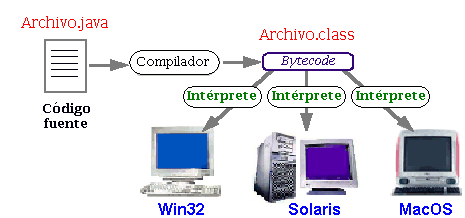
\includegraphics[scale=.65]{images/funcionamiento_java.png}
  \end{center}
\end{frame}  

\begin{frame}
  \frametitle{El Compilador {\texttt javac}}
  \framesubtitle{Ambiente de desarrollo Java}

  \begin{itemize}    
    \item Toma como entrada los archivos {\tt *.java} y configuraciones sobre el \emph{classpath}
    \item Genera archivos compilados en \emph{bytecode} en archivos {\tt *.class}      
    \item El \emph{classpath} indica dónde buscar otras clases
      externas a nuestro programa, tales como librerías
  \end{itemize}
\end{frame}

\begin{frame}
  \frametitle{La Máquina Virtual de Java --- JVM}

  Los archivos de bytecode son ejecutados por la JVM.

  \begin{itemize}
  \item La JVM carga el archivo de bytecode, y verifica qué este
    correctamente formado
    
  \item \textbf{Intérpretación inicial:} inicialmente el programa es
    ejecutado por el \emph{intérprete JVM}, que es una forma lenta de
    ejecutar, pero que puede partir de inmediato
    
  \item \textbf{Compilación Just-in-Time}: durante la ejecución, la
    JVM va progresivamente compilando al lenguaje máquina de la
    plataforma, para mejorar la velocidad de ejecución
    
  \end{itemize}
  
\end{frame}

\begin{frame}
  \frametitle{El Kit de Desarrollo --- JDK}

  \begin{exampleblock}{}
  Contiene las herramientas, programas, bibliotecas, y todos los
  elementos necesarios para el desarrollo y depuración de aplicaciones Java
  \end{exampleblock}

\end{frame}


\begin{frame}
  \frametitle{JDK / Compilación y Ejecución}  

  \begin{itemize}
    
  \item \texttt{javac}: es el compilador de Java, incluido solamente
    en el JDK. Se ejecuta desde línea de comandos: \texttt{javac HolaMundo.java}

  \item \texttt{java}: es el ejecutor de programas Java, se incluye
    tanto en el JDK como en el JRE. También se usa desde la línea de
    comandos: \texttt{javac HolaMundo.class}

  \item \texttt{javadoc}: Crea documentación en formato HTML a partir
    de el código fuente y los comentarios. Se usa desde la línea de
    comandos: \texttt{javadoc HolaMundo.java}    
    
  \end{itemize}

\end{frame}

\begin{frame}
  \frametitle{JDK / Utilitarios}

  \begin{itemize}
    
  \item \textt{jar}: crea librerías en formato JAR (Java ARChive), que
    permite empaquetar clases y otros recursos en un único paquete
    portable

  \item \texttt{jdb}: depurador de Java, con soporte para breakpoints
    y avance paso a paso. Se usa sobre archivos bytecode: \texttt {jdb
      HolaMundo 10} (10 es la linea del breakpoint). \emph{En general
      no se usa manualmente sino como parte de un editor integrado}
        
  \end{itemize}

\end{frame}
 
\begin{frame}[fragile]
  \frametitle{Hola Mundo en Java}

  \begin{java}{HolaMundo.java}
    public class HolaMundo {
      public static void main(String[] args) {
        System.out.println("Hola Mundo!");
      }
    }
  \end{java}

\end{frame}

\begin{frame}[fragile]
  \frametitle{Ejecutando Hola Mundo}

  \begin{bash}{Compilación y ejecución usando {\tt javac} y {\tt java}}
    > javac HolaMundo.java
    > java HolaMundo
    Hola Mundo!
  \end{bash}

\end{frame}


\subsection{Variables}

\begin{frame}
  \frametitle{Lenguajes de programación}
  \framesubtitle{Variables}

  {\scriptsize
    \begin{exampleblock}{Definición}
      \begin{itemize}
      \item Una \textbf{variable} es un \textbf{nombre} que contiene un valor que puede cambiar a lo largo del programa.
      \end{itemize}
    \end{exampleblock}

    \begin{block}{Tipos principales de variables}
      \begin{itemize}
      \item De acuerdo con el tipo de información que contienen, en JAVA hay dos tipos principales de variables:
        \begin{itemize}
        \item {\scriptsize Variables de \textbf{tipos primitivos}. Están definidas mediante un único valor que puede ser \textbf{entero}, de \textbf{punto flotante}, \textbf{carácter} o \textbf{booleano}. JAVA permite distinta \textbf{precición} y distintos rangos de valores para estos tipos de variables \textbf{char, byte, short, int, long, float, double, boolean}.}
        \item {\scriptsize Variables \textbf{referencia}. Las variables referencia son referencias o nombres de una información más compleja: \textbf{arrays} u \textbf{objetos} de una determinada clase.}
        \end{itemize}
      \end{itemize}
    \end{block}
  }
\end{frame}

\begin{frame}
  \frametitle{Lenguajes de programación}
  \framesubtitle{Variables}

  \begin{block}{Rol de las variables}
    \begin{itemize}
    \item Desde el punto de vista del rol o misión que cumplan en el programa, las variables pueden ser:
      \begin{itemize}
      \item Variables \textbf{miembros} de una clase. Se definen en una clase, fuera de cualquier método; pueden ser tipos primitivos o referencias. Comúnmente son llamados \textbf{atributos} de la clase.
      \item Variables \textbf{locales}. Se definen dentro de un método o más en general dentro de cualquier bloque entre llaves \{\}. Se crean en el interior del bloque y se destruyen al finalizar dicho bloque. Pueden ser también tipos primitivos o referencias.
      \end{itemize}
    \end{itemize}
  \end{block}
\end{frame}

\begin{frame}
  \frametitle{Lenguajes de programación}
  \framesubtitle{Variables - Nombres de variables}

  \begin{block}{Características de las variables}
    \begin{itemize}
    \item Los nombres de variables en JAVA se pueden crear con mucha libertad.
    \item Pueden ser cualquier conjunto de caracteres numéricos y alfanuméricos, sin algunos caracteres especiales utilizados por JAVA como operadores o separadores (\textbf{,.+-*/} etc).
    \item Existe una serie de palabras reservadas las cuales tienen un significado especial para JAVA y por lo tanto no se pueden utilizar como nombres de variables.
    \end{itemize}
  \end{block}
\end{frame}

\begin{frame}
  \frametitle{Lenguajes de programación}
  \framesubtitle{Variables - Palabras reservadas}

  \textbf{Palabras reservadas}
  \begin{center}
    \begin{tabular}{|c|c|c|c|c|c|} \hline
      abstract    & boolean & break         & byte                 & case     & catch        \\ \hline
      char          & class       & const*        & continue         & default & do              \\ \hline
      double     & else         & extends     & final                 & finally   & float \\ \hline
      for             & goto*       & if                 & implements    & import  & instanceof \\ \hline
      int             & interface  & long          & native              & new      & null \\ \hline
      package  & private     & protected & public              & return   & short \\ \hline
      static        & super       & switch       & synchronized & this       & throw \\ \hline
      throws      & transient & try              & void                  & volatile & while \\ \hline
    \end{tabular}
  \end{center}
  \textbf{(*)} son palabras reservadas, pero no se utilizan en la actual implementación del lenguaje JAVA
\end{frame}

\begin{frame}
  \frametitle{Lenguajes de programación}
  \framesubtitle{Variables -Tipos de datos primitivos}

  \begin{exampleblock}{Características de las variables}
    Se llaman \textbf{tipos primitivos} de variables de JAVA a aquellas variables sencillas que contienen los tipos de información más habituales: valores boolean, caracteres y valores numéricos enteros o de punto flotante. 
  \end{exampleblock}
  
  \begin{block}{Características de las variables}
    \begin{itemize}
    \item Java dispone de \textbf{ocho} tipos primitivos de variables:
      \begin{itemize}
      \item Un tipo para almacenar valores \textbf{true} y  \textbf{false}  \textbf{(boolean)}.
      \item Un tipo para almacenar \textbf{caracteres}  \textbf{(char)}.
      \item Seis tipos para guardar valores \textbf{numéricos}.
        \begin{itemize}
        \item Cuatro tipos para \textbf{enteros} \textbf{(byte, short, int y long)}
        \item Dos para valores \textbf{reales de punto flotante} \textbf{(float y double)}.
        \end{itemize}
      \end{itemize}
    \end{itemize}
  \end{block}
\end{frame}

\begin{frame}
  \frametitle{Lenguajes de programación} 
  \framesubtitle{Variables -Tipos de datos primitivos}

  {\scriptsize
    \begin{center}
      \begin{tabular}{|l|l|l|} \hline
        \multicolumn{1}{|>{\columncolor[rgb]{0.8, 0.8, 0.8}}l|}{\textbf{Tipo de variable}} &
                                                                                             \multicolumn{1}{|>{\columncolor[rgb]{0.8, 0.8, 0.8}}l|}{\textbf{Descripción}} \\ \hline
        \textbf{boolean} & 1 byte. Valores true y false. \\ \hline
        \textbf{char} 	 & 2 bytes. Unicode. Comprende el código ASCII. \\ \hline
        \textbf{byte} 	 & 1 byte. Valor entero entre -128 y 127. \\ \hline
        \textbf{Short} 	 & 2 bytes. Valor entero entre -32768 y 32767. \\ \hline
        \textbf{int}		 & 4 bytes. Valor entero entre -2.147.483.648 y
        \\ 			 & 2.147.483.647. \\ \hline
        \textbf{long} 	 & 8 bytes. Valor entre -9.223.372.036.854.775.808 y
        \\			 & 9.223.372.036.854.775.807. \\ \hline
        \textbf{float}	 & 4 bytes (entre 6 y 7 cifras decimales equivalentes). 
        \\ 			 & De -3.402823E38 a -1.401298E-45 y de 1.401298E-45 a 
        \\			 & 3.402823E38. \\ \hline
        \textbf{double}	 & 8 bytes (unas 15 cifras decimales equivalentes). 
        \\ 			 & De -1.79769313486232E308 a -4.94065645841247E-324
        \\ 			 & y de 4.94065645841247E-324 a 1.79769313486232E308. \\ \hline
      \end{tabular}
    \end{center}
  }
\end{frame}

\begin{frame}
  \frametitle{Lenguajes de programación} 
  \framesubtitle{Variables -Tipos de datos primitivos}

  Los tipos primitivos de JAVA tienen algunas características importantes:

  \begin{itemize}
  \item El tipo \textbf{boolean} no es un valor numérico.
    \begin{itemize}
    \item Sólo admite los valores \textbf{true} o \textbf{false}. 
    \item El tipo boolean no se identifica con el igual o distinto de cero, como en otros lenguajes.
    \item El resultado de la expresión lógica que aparece como condición en un bucle o en una bifurcación debe ser boolean.
    \end{itemize}
  \item El tipo \textbf{char} contiene caracteres en código UNICODE (que incluye el código ASCII), y ocupan 16 bits (2 bytes) por carácter. Comprende los caracteres de prácticamente todos los idiomas.
  \end{itemize}
\end{frame}

\begin{frame}
  \frametitle{Lenguajes de programación} 
  \framesubtitle{Variables -Tipos de datos primitivos}

  Los tipos primitivos de JAVA tienen algunas características importantes:

  \begin{itemize}
  \item Los tipos \textbf{byte, short, int y long} son números enteros que pueden ser positivos o negativos, con distintos valores máximos y mínimos. A diferencia de otros lenguajes, en JAVA no hay enteros \textbf{unsigned}.
  \item Los tipos \textbf{float} y \textbf{double} son valores de punto flotante (números reales) con 6-7 y 15 cifras decimales exactas (significativos), respectivamente.
  \item Se utiliza la palabra 	\textbf{void} para indicar la ausencia de un tipo de variable determinado.
  \end{itemize}
\end{frame}

\begin{frame}
  \frametitle{Lenguajes de programación} 
  \framesubtitle{Variables -Tipos de datos primitivos}

  Los tipos primitivos de JAVA tienen algunas características importantes:

  \begin{itemize}
  \item A diferencia de otros lenguajes, los tipos de variables en JAVA están perfectamente definidos en todas y cada una de las posibles plataformas. Por ejemplo, un int ocupa siempre la misma memoria y tiene el mismo rango de valores, en cualquier tipo de ordenador.
  \item Existen extensiones de JAVA para aprovechar la arquitectura de los procesadores Intel, que permiten realizar operaciones de punto flotente con una precisión extendida de 80 bits (10 bytes).
  \end{itemize}
\end{frame}

\begin{frame}
  \frametitle{Lenguajes de programación} 
  \framesubtitle{Variables - Definición de variables}

  Definición de variables en JAVA.

  \begin{itemize}
  \item Una variable se define especificando el tipo y el nombre de dicha variable.
  \item Estas variables pueden ser tanto de tipos primitivos como referencias a objetos de alguna clase.
  \item Si no se especifica un valor en su declaración, las variables primitivas deberán ser inicializadas antes de su uso, sino, JAVA no reconocerá la variable en el contexto actual.
  \end{itemize}
\end{frame}

\begin{frame}
  \frametitle{Lenguajes de programación} 
  \framesubtitle{Variables - Definición de variables}

  Definición de variables en JAVA.

  \begin{itemize}
  \item Es importante distinguir entre la \textbf{referencia} a un objeto y el \textbf{objeto} mismo.
  \item Una referencia es una variable que indica dónde está guardado un objeto en la memoria del ordenador.
    \begin{itemize}
    \item A diferencia de otros lenguajes, JAVA no permite acceder al valor de la dirección, pues en este lenguaje se han eliminado los \textbf{punteros}.
    \end{itemize}
  \item Al declarar una referencia, ésta aún no se encuentra ''apuntando'' a ningún objeto en particular y por eso se le asigna el valor \textbf{null}.
  \item Si se desea que esta referencia apunte a un nuevo objeto es necesario crear el objeto utilizando el operador \textbf{new}. Este operador reserva en la memoria del ordenador espacio para ese objeto. 
  \end{itemize}
\end{frame}

\begin{frame}
  \frametitle{Lenguajes de programación} 
  \framesubtitle{Variables - Visibilidad y vida de las variables}

  \begin{block}{Definición}
    \begin{itemize}
    \item Se entiende por \textbf{visibilidad, ámbito, alcance o scope} de una variable, el fragmento o parte de la aplicación donde dicha variable es accesible y por lo tanto puede ser utilizada en una expresión.
    \item En JAVA todas las variables deben estar incluidas en una clase.
    \item En general las variables declaradas dentro de unas llaves \{\}, es decir dentro de un bloque, son visibles y existen dentro de estas llaves. 
    \end{itemize}
  \end{block}
\end{frame}

\subsection{Operadores}

\begin{frame}
  \frametitle{Lenguajes de programación} 
  \framesubtitle{Operadores - Aritméticos}

  \begin{block}{Operadores aritméticos}
    \begin{itemize}
    \item[$\rightarrow$] Son operadores binarios (requieren siempre dos operandos) que realizan las operaciones aritméticas habituales: \textbf{suma} (+), \textbf{resta} (-), \textbf{multiplicación} (*), \textbf{división} (/) y \textbf{resto de la división} (\%).
    \end{itemize}
  \end{block}
\end{frame}

\begin{frame}
  \frametitle{Lenguajes de programación} 
  \framesubtitle{Operadores - Asignación}

  \begin{block}{Operadores de asignación}
    \begin{itemize}
    \item Los operadores de asignación permiten asignar un valor a una variable.
    \item El operador de asignación por excelencia es el operador \textbf{igual} (=). 
    \item La forma general de las sentencias de asignación con este operador es:
      \begin{itemize}
      \item \textbf{variable} = \textbf{expresion};
      \end{itemize}
    \item JAVA dispone de otros operadores de asignación. Se trata de las versiones abreviadas del operador (=) que realizan operaciones ''acumulativas'' sobre una variable.
    \end{itemize}
  \end{block}
\end{frame}

\begin{frame}
  \frametitle{Lenguajes de programación} 
  \framesubtitle{Operadores - Asignación acumulativas}

  \begin{center}
    \begin{tabular}{|l|l|l|} \hline
      \multicolumn{1}{|>{\columncolor[rgb]{0.8, 0.8, 0.8}}c|}{\textbf{Operador}} &
                                                                                   \multicolumn{1}{|>{\columncolor[rgb]{0.8, 0.8, 0.8}}c|}{\textbf{Uso}} &
                                                                                                                                                           \multicolumn{1}{|>{\columncolor[rgb]{0.8, 0.8, 0.8}}c|}{\textbf{Expesión equivalente}} \\ \hline
      \textbf{$+=$}	& op1 \textbf{$+=$} op2 	& op1 $=$ op1 $+$ op2 \\ \hline
      \textbf{$-=$}	& op1 \textbf{$-=$} op2 	& op1 $=$ op1 $-$ op2  \\ \hline
      \textbf{$*=$} 	& op1 \textbf{$*=$} op2 	& op1 $=$ op1 $*$ op2  \\ \hline
      \textbf{$/=$}	& op1 \textbf{$/=$} op2 	& op1 $=$ op1 $/$ op2  \\ \hline
      \textbf{$\%=$}	& op1 \textbf{$\%=$} op2 	& op1 $=$ op1 $\%$ op2  \\ \hline
    \end{tabular}
  \end{center}
\end{frame}

\begin{frame}
  \frametitle{Lenguajes de programación} 
  \framesubtitle{Operadores - Unarios e Instanceof}

  \begin{block}{Operadores unarios}
    Los operadores \textbf{más} (+) y \textbf{menos} (-) unarios sirven para mantener o cambiar el signo de una variable o expresión numérica.
  \end{block}

  \begin{block}{Operador \textbf{instanceof}}
    \begin{itemize}
    \item El operador \textbf{instanceof} permite saber si un objeto pertenece o no a una determinada clase.
    \item Es un operador binario cuya forma general es:
      \begin{itemize}
      \item objectName \textbf{instanceof} ClassName
      \end{itemize}
    \item Devuelve \textbf{true o false} según el objeto pertenezca o no a la clase.
    \end{itemize}
  \end{block}
\end{frame}

\begin{frame}
  \frametitle{Lenguajes de programación} 
  \framesubtitle{Operadores - Condicional \textbf{?}}

  \begin{block}{Operador condicional \textbf{?}}
    \begin{itemize}
    \item Este operador permite realizar bifurcaciones condicionales sencillas.
    \item Su forma general es la siguiente:
      \begin{itemize}
      \item expresionBooleana \textbf{?} respExpresionVerdero : respExpresionFalso
      \end{itemize}
    \item Se evalúa \textbf{expresionBooleana} y devuelve \textbf{respExpresionVerdero} si es verdadera o \textbf{respExpresionFalso} si es falsa.
    \item Es el único operador ternario en JAVA (requiere de tres argumentos).
    \end{itemize}
  \end{block}
\end{frame}

\begin{frame}
  \frametitle{Lenguajes de programación} 
  \framesubtitle{Operadores - Incrementales}

  \begin{block}{Operadores incrementales}
    \begin{itemize}
    \item JAVA dispone del operador \textbf{incremento} ($++$) y \textbf{decremento} ($- -$).
    \item El operador ($++$) incrementa en una unidad la variable a la que se aplica, mientras que ($- -$) la reduce en una unidad.
    \item Estos operadores se pueden utilizar de dos formas:
      \begin{itemize}
      \item \textbf{Precediendo}  a la variable \textbf{($++x$)}. En este caso primero se utiliza la variable en la expresión (con el valor actual) y luego se incrementa.
      \item \textbf{Siguiendo} a la variable \textbf{($x++$)}. En este caso primero se incrementa la variable y luego se utiliza (ya incrementada) en la expresión en la que aparece.
      \end{itemize}
    \end{itemize}
  \end{block}
\end{frame}

\begin{frame}
  \frametitle{Lenguajes de programación} 
  \framesubtitle{Operadores - Relacionales}

  \begin{block}{Operadores relacionales}
    \begin{itemize}
    \item Los operadores relacionales sirven para realizar comparaciones de igualdad, desigualdad y relación de menor o mayor. 
    \item El resultado de estos operadores es siempre un valor \textbf{boolean (true o false)} según se cumpla o no la relación considerada. 
    \item Estos operadores se utilizan con mucha frecuencia en las \textbf{bifurcaciones} y en los \textbf{bucles}.
    \end{itemize}
  \end{block}
\end{frame}

\begin{frame}
  \frametitle{Lenguajes de programación} 
  \framesubtitle{Operadores - Relacionales}

  \begin{center}
    \begin{tabular}{|l|l|l|} \hline
      \multicolumn{1}{|>{\columncolor[rgb]{0.8, 0.8, 0.8}}c|}{\textbf{Operador}} &
                                                                                   \multicolumn{1}{|>{\columncolor[rgb]{0.8, 0.8, 0.8}}c|}{\textbf{Uso}} &
                                                                                                                                                           \multicolumn{1}{|>{\columncolor[rgb]{0.8, 0.8, 0.8}}c|}{\textbf{El resultado es true si:}} \\ \hline
      \textbf{$>$}	& op1 \textbf{$>$} op2 	& op1 es mayor que op2 \\ \hline
      \textbf{$>=$}	& op1 \textbf{$>=$} op2 	& op1 es mayor o igual que op2 \\ \hline
      \textbf{$<$} 	& op1 \textbf{$<$} op2 	& op1 es menor que op2\\ \hline
      \textbf{$<=$}	& op1 \textbf{$<=$} op2 	& op1 es mayor o igual que op2 \\ \hline
      \textbf{$==$}	& op1 \textbf{$==$} op2 	& op1 y op2 son iguales \\ \hline
      \textbf{$!=$}	& op1 \textbf{$!=$} op2 	& op1 y op2 son diferentes \\ \hline
    \end{tabular}
  \end{center}
\end{frame}

\begin{frame}
  \frametitle{Lenguajes de programación} 
  \framesubtitle{Operadores - Lógicos}

  \begin{block}{Operadores lógicos}
    \begin{itemize}
    \item Los operadores lógicos se utilizan para construir expresiones lógicas, combinando valores lógicos \textbf{(true y/o false)} o los resultados de los operadores relacionales. 
    \item Debe notarse que en ciertos casos el segundo operando no se evalúa porque ya no es necesario (si ambos tienen que ser true y el primero es false, ya se sabe que la condición de que ambos sean true no se va a cumplir). 
    \item Esto puede traer resultados no deseados y por eso se han a\~nadido los operadores (\textbf{\&}) y (\textbf{$\mid$}) que garantizan que los dos operandos se evalúan siempre.
    \end{itemize}
  \end{block}
\end{frame}

\begin{frame}
  \frametitle{Lenguajes de programación} 
  \framesubtitle{Operadores - Lógicos}

  {\scriptsize
    \begin{center}
      \begin{tabular}{|l|l|l|l|} \hline
        \multicolumn{1}{|>{\columncolor[rgb]{0.8, 0.8, 0.8}}c|}{\textbf{Operador}} &
                                                                                     \multicolumn{1}{|>{\columncolor[rgb]{0.8, 0.8, 0.8}}c|}{\textbf{Nombre}} &
                                                                                                                                                                \multicolumn{1}{|>{\columncolor[rgb]{0.8, 0.8, 0.8}}c|}{\textbf{Uso}} &
                                                                                                                                                                                                                                        \multicolumn{1}{|>{\columncolor[rgb]{0.8, 0.8, 0.8}}c|}{\textbf{Resultado es true si:}}  \\ \hline
        \textbf{\&\&}		& AND 		& op1 \textbf{\&\&} op2 		& op1 y op2 son true. Si op1 es false 
        \\				&			&						& ya no se evalúa op2. \\ \hline
        \textbf{$\mid\mid$}	& OR 		& op1 \textbf{$\mid\mid$} op2 	& op1 y op2 son true. Si op1 es verdadero 
        \\				&			&						& ya no se evalúa op2 \\ \hline
        \textbf{$!=$}		& Negación 	& \textbf{$!$} op 			& op es falso y es falso si op es verdadero 
        \\				&			&						& ya no se evalúa op2 \\ \hline
        \textbf{\&}			& AND 		& op1 \textbf{\&} op2 		& op1 y op2 son true. Siempre se evalúa op2. \\ \hline
        \textbf{$\mid$}		& OR 		& op1 \textbf{$\mid$}	 op2 		& op1 u op2 son true.  Siempre se evalúa op2. \\ \hline
      \end{tabular}
    \end{center}
  }
\end{frame}

\begin{frame}
  \frametitle{Lenguajes de programación} 
  \framesubtitle{Operadores - Concatenación de caracteres}

  \begin{block}{Operador de concatenación de caráteres}
    \begin{itemize}
    \item El operador \textbf{más (+)} se utiliza también para concatenar cadenas de caracteres.
    \item Por ejemplo, para escribir una cantidad con un rótulo y unas unidades puede utilizarse la sentencia:
      \begin{itemize}
      \item System.out.println(''El total asciende a '' \textbf{+} totalUnidades );
      \end{itemize}
    \item En el ejemplo anterior, el operador de concatenación se utiliza para construir la cadena de caracteres que se desea imprimir por medio del mótodo \textbf{println()}.
    \item La variable numérica \textbf{totalUnidades} es convertida automáticamente por JAVA en cadena de caracteres para poderla concatenar. En otras ocasiones se deberá llamar explícitamente a un método para que realice esta conversión.
    \end{itemize}
  \end{block}
\end{frame}

\subsection{Estructuras de control}

\begin{frame}
  \frametitle{Lenguajes de programación}
  \framesubtitle{Estructuras de control}

  {\scriptsize
    \begin{block}{Definición}
      \begin{itemize}
      \item Facilitan la realización de determinadas acciones, mientras que una condición se cumpla. 
      \item Permiten tomar decisiones de \textbf{qué} hacer, en función de las condiciones que se den en el programa en un momento dado de su ejecución.
      \end{itemize}
    \end{block}
    \begin{exampleblock}{En JAVA}
      El lenguaje JAVA soporte cuatro tipos de estructuras de control:
      \begin{itemize}
      \item \textbf{Toma de decisión:} if / if-else / switch-case.
      \item \textbf{Bucle o ciclo:} for / while / do-while.
      \item \textbf{Saltos:} break / continue / return / goto.
      \item \textbf{Excepciones.}
      \end{itemize}
    \end{exampleblock}
  }
\end{frame}

\begin{frame}
  \frametitle{Lenguajes de programación}
  \framesubtitle{Estructuras de control - Sentencias condicionales}

  \begin{itemize}
  \item En JAVA la sentencia \textbf{if / if-else}  dota a los programas de la habilidad de ejecutar conjuntos de sentencias según la condición.
  \end{itemize}

  \begin{block}{La sentencia para \textbf{if} es:}
    {\scriptsize
      \textbf{if} (condición) \textbf{\{} \\
      \hspace{0.3cm} Bloque de sentencias si la condición es \textbf{verdadera}.  \\
      \textbf{\}}
    }
  \end{block}

  \begin{block}{La sentencia para \textbf{if-else} es:}
    {\scriptsize
      \textbf{if} (condición) \textbf{\{} \\
      \hspace{0.3cm} Bloque de sentencias si la condición es \textbf{verdadera}.  \\
      \textbf{\}}\\
      \textbf{else \{}\\
      \hspace{0.3cm} Bloque de sentencias si la condición es \textbf{falsa}.  \\
      \textbf{\}}
    }
  \end{block}
\end{frame}

\begin{frame}
  \frametitle{Lenguajes de programación}
  \framesubtitle{Estructuras de control - Sentencias condicionales}

  \begin{itemize}
  \item Supongamos que un programa debe realizar diferentes acciones dependiendo de si el usuario oprime el botón \textbf{aceptar} o el botón \textbf{cancelar} en una ventana de diálogo. Nuestro programa puede realizar esta bifurcación usando la sentencia \textbf{if-else}:
  \end{itemize}
  
  \begin{block}{Bifurcación con la sentencia \textbf{if-else}.}
    {\scriptsize
      \textbf{if} (respuesta.equals(''Aceptar'')) \textbf{\{} \\
      \hspace{0.3cm} System.out.println(''Su petición esta siendo atendida'');  \\
      \textbf{\}}\\
      \textbf{else \{}\\
      \hspace{0.3cm} System.out.println(''Cancelando acción'' );  \\
      \textbf{\}}
    }
  \end{block}
\end{frame}

\begin{frame}
  \frametitle{Lenguajes de programación}
  \framesubtitle{Estructuras de control - Sentencias condicionales}

  \begin{itemize}
  \item Se pueden anidar expresiones \textbf{if-else}, para poder implementar aquellos casos con múltiples acciones. Esto es lo que se suele denominar como sentencias \textbf{else-if}.
  \end{itemize}

  \begin{block}{Ejemplo de Bifurcaciones múltiples:}
    \begin{itemize}
    \item Supongamos que se desea escribir un programa que clasifique según el contenido de una variable denominada \textbf{valor}, asigne una letra a otra variable denominada \textbf{clasificacion}.
    \item A, para un valor entre 100 y 91 (inclusive).
    \item B, para un valor entre 90 y 81 (inclusive).
    \item C, para un valor entre 80 y 71 (inclusive).
    \item F, si no es ninguno de los anteriores.
    \end{itemize}
  \end{block}
\end{frame}

\begin{frame}
  \frametitle{Lenguajes de programación}
  \framesubtitle{Estructuras de control - Sentencias condicionales}

  \begin{block}{Ejemplo de Bifurcaciones múltiples - Solución}
    {\scriptsize
      \textbf{int} valor;\\
      \textbf{char} clasificacion;\\
      \vspace{0.3cm}
      \textbf{if} (valor $>$ 90 \hspace{0.1cm} \textbf{\&\&} \hspace{0.1cm} valor $<=$ 100) \textbf{\{} \\
      \hspace{0.3cm} clasificacion = 'A';\\
      \textbf{\}} \\
      \textbf{else if} (valor $>$ 80 \hspace{0.1cm} \textbf{\&\&} \hspace{0.1cm} valor $<$= 90) \textbf{\{} \\
      \hspace{0.3cm} clasificacion = 'B';\\
      \textbf{\}} \\
      \textbf{else if} (valor $>$ 70 \hspace{0.1cm} \textbf{\&\&} \hspace{0.1cm} valor $<$= 80) \textbf{\{} \\
      \hspace{0.3cm} clasificacion = 'C';\\
      \textbf{\}} \\
      \textbf{else} \textbf{\{} \\
      \hspace{0.3cm} clasificacion = 'F';\\
      \textbf{\}}
    }
  \end{block}
\end{frame}

\begin{frame}
  \frametitle{Lenguajes de programación}
  \framesubtitle{Estructuras de control - Sentencias condicionales}

  \begin{itemize}
  \item Este sistema de programación (else-if) no es recomendable, por la pérdida de claridad en la lectura del programa. Por ello el lenguaje JAVA incluye la sentencia \textbf{switch-case}, para dirigir el flujo de control de variables con múltiples valores.
  \item La sentencia \textbf{switch} permite seleccionar entre varias opciones, según el valor de cierta expresión.
  \item Cada sentencia case debe ser única y el valor que evalúa debe ser del mismo tipo que el devuelto por la expresión de la sentencia \textbf{switch}.
  \item Las sentencias \textbf{break} permiten salir del \textbf{switch} y continar con la siguiente instrucción. Las sentencias \textbf{break} son necesarias porque sin ellas se ejecutarían secuencialmente las sentencias \textbf{case} restantes. 
  \end{itemize}
\end{frame}

\begin{frame}
  \frametitle{Lenguajes de programación}
  \framesubtitle{Estructuras de control - Sentencias condicionales}

  \begin{itemize}
  \item Finalmente, se puede usar la sentencia \textbf{default} para manejar los valores que no son explícitamente contemplados por alguna de las sentencias \textbf{case}. Su uso es altamente recomendado.
  \end{itemize}

  \begin{block}{La forma general de la sentencia \textbf{switch} es la siguiente:}
    {\scriptsize
      \textbf{switch} (expresionMultivalor) \textbf{\{} \\
      \hspace{0.3cm} \textbf{case} valor1: \\
      \hspace{0.6cm} bloqueDeSentenciasParaValor1; \\
      \hspace{0.6cm} \textbf{break}; \\
      \hspace{0.3cm} \textbf{case} valor2: \\
      \hspace{0.6cm} bloqueDeSentenciasParaValor2; \\
      \hspace{0.6cm} \textbf{break}; \\
      \hspace{0.3cm}...\\
      \hspace{0.3cm} \textbf{default}: \\
      \hspace{0.6cm} bloqueDeSentenciasParaValorNoDeterminado; \\
      \hspace{0.6cm} \textbf{break}; \\
      \textbf{\}}
    }
  \end{block}
\end{frame}

\begin{frame}
  \frametitle{Lenguajes de programación}
  \framesubtitle{Estructuras de control - Sentencias condicionales}

  \begin{block}{Ejemplo de sentencia \textbf{switch}}
    \begin{itemize}
    \item Supongamos un programa con una variable entera \textbf{meses} cuyo valor indica el mes actual y se desea imprimir el nombre del mes en que estemos. Se puede utilizar la sentencia \textbf{switch} para realizar esta operación.
    \item Si el valor a comparar no existe o no es un valor válido, el programa debe indicar el error.
    \item Luego de implementar la solución con la sentencia \textbf{switch}, implementarla con la sentencia \textbf{else-if} y comparar ambas soluciones. 
    \end{itemize}
  \end{block}
\end{frame}

\begin{frame}
  \frametitle{Lenguajes de programación}
  \framesubtitle{Estructuras de control - Sentencias condicionales}

  \begin{block}{Ejemplo de sentencia \textbf{switch} - Solución}
    {\scriptsize
      \textbf{int} mes;\\
      \vspace{0.3cm}
      \textbf{switch} (mes) \textbf{\{} \\
      \hspace{0.3cm} \textbf{case} 1: \\
      \hspace{0.6cm} System.out.println(''Enero''); \\
      \hspace{0.6cm} \textbf{break}; \\
      \hspace{0.3cm} \textbf{case} 2: \\
      \hspace{0.6cm} System.out.println(''Febrero''); \\
      \hspace{0.6cm} \textbf{break}; \\
      \hspace{0.3cm} //... Otros meses \\
      \hspace{0.3cm} \textbf{default}: \\
      \hspace{0.6cm} System.out.println(''Mes no válido''); \\
      \hspace{0.6cm} \textbf{break}; \\
      \textbf{\}}
    }
  \end{block}
\end{frame}

\begin{frame}
  \frametitle{Preguntas}
  \hspace{4cm}\huge{Preguntas ?}  
\end{frame}

\end{document}
